\documentclass[twocolumn,10pt,a4paper]{article}

\usepackage{graphicx}
\usepackage{amsmath,amssymb,mathtools,bm}
\usepackage{braket}
\usepackage{hyperref}
\usepackage[version=4]{mhchem}
\usepackage{authblk}
\usepackage{siunitx}
\usepackage{physics}
\usepackage[utf8]{inputenc}
\usepackage[T1]{fontenc}
\usepackage{abstract}     
\usepackage{geometry}    
\usepackage{cite}       
\usepackage{multicol}
\usepackage[font=small, labelfont=bf]{caption}
\usepackage{float}
\title{Experimental evidence for 3D topological insulators using Weak Anti-localization and the Quantum Hall Effect}
\author{Taliko Hofmann}
\affil{Department of Physics, University of W\"urzburg}
\date{\today}

\begin{document}

\twocolumn[
\maketitle
\begin{abstract}
    Three-dimensional topological insulators (3DTIs) host insulating bulk states and conducting topological surface states, described by spin-momentum locked Dirac fermions. While angle-resolved photoemission spectroscopy experiments can identify these topological surface states, transport measurements on these surface states remain a challenge, due to residual bulk conduction and disorder effects. This seminar paper reviews two widely used methods for probing electronic transport in 3DTIs, namely weak-antilocalization (WAL) and the quantum Hall effect (QHE). First WAL experiments by García-Abad \textit{et al.}~\cite{nano11051077} and Li \textit{et al.}~\cite{Li}. Then QHE experiments from Hartl \textit{et al.}~\cite{Hartl} and Xu \textit{et al.}~\cite{Xu_2014} are reviewed, both of which observe well quantized Hall plateaus and vanishing longitudinal resistances. These approaches offer compelling experimental evidence of surface state dominated electronic transport in 3DTIs, for certain film thicknesses and temperature regimes. 
\end{abstract}
]
\section{Introduction and Theory}
\label{sec:intro}
Two-dimensional topological insulators were first confirmed experimentally in 2007~\cite{Konig2007}, with their three-dimensional counterparts shortly after in 2008~\cite{Hsieh2008}. Topological insulators are characterized by an insulating bulk state with a gapped energy spectrum, and gapless, metallic surface states that carry charges dissipationlessly. The surface states of topological insulators are typically attributed to band inversion. Because of their special topology, such systems possess surface states, which are robust against local perturbations, making them prominent candidates for novel electronic devices. The surface states in 3DTIs can be described by two-dimensional Dirac fermions experiencing strong spin-orbit coupling (SOC). The SOC locks the electron's momentum to its spin orientation, leading to a $\pi$ Berry phase when the electron adiabatically completes a time-reversed, self-intersecting path in the quantum diffusive regime (see Fig.~\ref{fig:diffusiveregime})~\cite{Competition}. While the topological surface states have been observed by spectroscopic techniques such as angle resolved photoemission spectroscopy (ARPES), it remains a challenge to study the electronic transport in these materials. This difficulty arises due to a significant contribution from bulk charge carriers~\cite{nano11051077}. It is also important to consider the contribution from the interplay of different charge-carrier species on the different surfaces of the sample~\cite{Hartl}. In this seminar paper two methods, used to investigate the electronic transport in 3DTIs are introduced in the next chapter. The first method to be presented is weak anti-localization (WAL) followed by the quantum Hall effect (QHE). In the subsequent chapter a selection of papers, serving as example experiments that employ the previously introduced methods, are examined and their methods are analyzed. 
\begin{figure}[h]
\centering
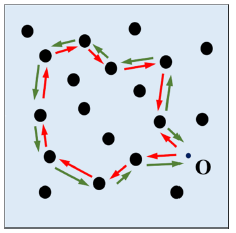
\includegraphics[width=0.4\textwidth]{figures/quantum_diffusive_regime.png}
\caption{Illustration of the quantum diffusive regime. Picture taken from~\cite{Lu_2014} Fig. 4(b).}
\label{fig:diffusiveregime}
\end{figure}
\subsection{Weak Anti-Localization}
\label{sec:WAL}
Weak anti-localization is a quantum interference effect, introducing a quantum correction to the classical conductivity $\sigma$. In order to observe this effect, the electronic transport needs to be in the quantum diffusive regime characterized by $l_\Phi \simeq L \gg l$, with the phase coherence length $l_\Phi$, the system size $L$, and the mean free path $l$. Because of the non-trivial $\pi$ Berry phase, destructive interference can suppress backscattering of surface electrons, therefore leading to an increase of $\sigma$~\cite{Lu_2014}. WAL only occurs if time reversal symmetry (TRS) is present. Therefore, WAL can be detected by breaking TRS via application of an external magnetic field $B$ and measuring $\sigma$ across a range of magnetic fields. A decrease in magnetoconductivity for an increasing field strength $|B|$ indicates WAL (see Fig.~\ref{fig:alpha_over_t}(d)). 
\subsection{Quantum Hall Effect}
\label{sec:QHE}
The quantum Hall effect is a topological state that is characterized by a quantized Hall resistance $R_{xy}$ and a vanishing longitudinal resistance $R_{xx}$ (see Fig.\@~\ref{fig:hartl_hall_resistance}) and is a hallmark signature of two-dimensional electron systems (2DES). The vanishing $R_{xx}$ is explained by one-dimensional chiral edge modes driven by cyclotron motion of two-dimensional electrons that carry charge dissipationlessly~\cite{Yoshimi2015}. The plateaus of $R_{xy}$ arise from the quantization of electron motion into  Landau levels (LLs), occurring when an integer number of LLs are completely filled. For the integer QHE $R_{xy} = h/(e^2 \nu)$, where $h$ is the Planck constant, $e$ the elementary charge, and $\nu \in \mathbb{N}$ is the LL filling factor, corresponding to the number of completely filled LLs. In the case of 3DTIs, a filling factor given by the sum of the contributions of the parallel conducting top and bottom surfaces $\nu=(\nu_\mathrm{t}+\nu_\mathrm{b})$~\cite{Xu_2014}. Because 2DES exhibit quantized Hall conductance, the observation of quantized plateaus in 3DTIs serves as strong evidence that transport is dominated by surface states. Since bulk conduction tends to suppress quantization, the QHE is a great tool for isolating and characterizing the contribution of topological surface channels to the electronic transport.
\section{WAL Experiments}
\label{sec:WAL ex}
In this section two papers measuring WAL are discussed. The first experiment by Garcia-Abad \textit{et al.}\@~\cite{nano11051077}, investigates thin film 3DTIs made out of $Bi_2Se_3$ with thicknesses $t$ ranging from a few quintuple layers ($1\,$QL $\simeq 1\,$nm) to several micrometers. The authors use the Hikami-Larkin-Nagaoka (HLN) model to calculate the conductance variation coming from WAL, which is given by 
~\begin{align}
\Delta \sigma(B) 
&= \frac{\alpha e^2}{2\pi^2 \hbar} \left[ 
\psi \left( \frac{1}{2} + \frac{\hbar}{4eB l_\phi^2} \right) \right. \nonumber \\
&\quad \left. -\ln \left( \frac{\hbar}{4eB l_\phi^2} \right)\right].
\label{HLN}
\end{align}
Here, $l_\phi$ is the phase coherence length, $\psi$ is the digamma function, $e$ the electronic charge, $\hbar$ the reduced Planck constant. The SOC-parameter $\alpha$ characterizes the number and nature of coherent conducting channels. Each decoupled 2D channel contributes $-1/2$. For ideal $Bi_2Se_3$ thin films with decoupled top and bottom surfaces, one expects $\alpha = -1$. However, values of around $\alpha = -1/2$ are commonly observed, which indicates that top- and bottom-surface states are indirectly coupled through the conducting bulk~\cite{nano11051077}. The authors compare several experiments to show how $\alpha$ and $l_\phi$ behave for different film thicknesses and sample qualities. They do this by fitting the measured magnetoresistance curves using eq.\ref{HLN} and treating $l_\phi$ and $\alpha$ as free parameters. They then compare the obtained values for different sample quality and plot them for different thicknesses. 
For example, in Bi$_2$Se$_3$ films grown by molecular beam epitaxy (MBE) on sapphire (Ref.~[13] in~\cite{nano11051077}), $\alpha \simeq -1/2$ for thicknesses above 6 QL, but drops to zero for ultrathin films below this threshold (see Fig.~\ref{fig:alpha_over_t}). This is explained by direct coupling between the top and bottom surface states. The surface contribution to conduction increases as the film becomes thinner (see Fig. 6(a) in~\cite{nano11051077}), but vanishes for $t<5\,$QL, while $l_\phi$ increases with increasing $t$. 
\begin{figure}[h]
\centering
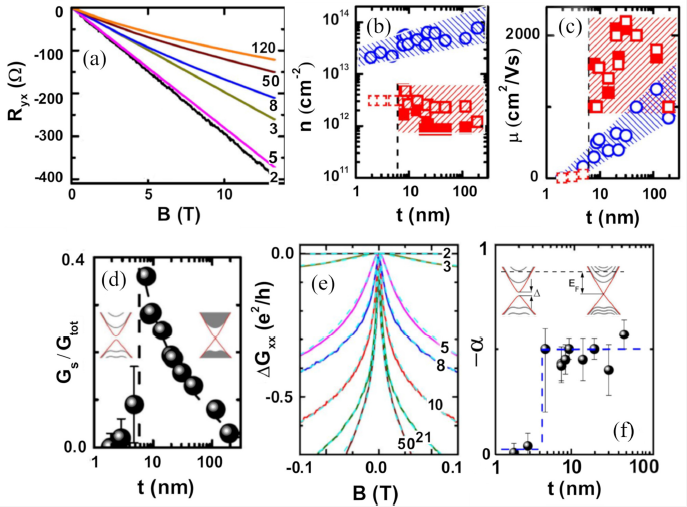
\includegraphics[width=\linewidth]{figures/ruben_1.png}
\caption{Here Fig.6 in~\cite{nano11051077} can be seen.(a) $R_{xy}$ against $B$ for different thicknesses, given in QL. A non-linear dependence can be observed.(b)+(c) Blue circles correspond to the bulk data and red squares correspond to the surface data (empty and filled implying both surfaces).(d) Surface conductance $G_s$ divided by total conductance $G_{tot}$ plotted over film thickness.(e) 2D magnetoconductance plotted over different film thicknesses.(f) Fitting parameter $\alpha$ plotted over film thickness $t$. At the critical thickness of $5$QL $\alpha$ abruptly drops to $0$, indicating small to none surface transport.}
\label{fig:alpha_over_t}
\end{figure}
On the other hand, in cleaner MBE-grown samples, pure surface transport can be realized, as reported in Ref.~[64] in~\cite{nano11051077}. For these samples, $l_\phi$ remains constant for thicknesses above $\sim$8 QL, consistent with dominant 2D surface conduction, while $\alpha$ ranges between $-1/2$ to $-1$. Deviations of $\alpha$ from $-1$ or $-1/2$ may arise from complex interactions between the surface states and a two-dimensional electron gas present because of band bending, attributed to environmental exposure~\cite{BRAHLEK201554}. However, this is only achieved under very specific growth conditions and with suppressed bulk doping, which, along with gating, is necessary to observe topological states. 
Other experiments (Ref.~[31] in~\cite{nano11051077}) show that in thick, bulk conduction dominated films, $\alpha$ remains near $-1/2$. This can either be attributed to WAL originating from the bulk or by a single channel composed of two surfaces coupled through the bulk~\cite{nano11051077}. But since $l_\phi$ increases with thickness approximately as $l_\phi \propto t^{0.7}$, . For samples with a high impurity concentration, $l_\phi$ reaches a linear dependence, indicating transport completely dominated by bulk carriers.
In conclusion the study by Garcia-Abad \textit{et al.} demonstrates that WAL is a universal phenomenon in $Bi_2Se_3$ films, even when bulk carriers dominate the transport. Although values of $\alpha \simeq -1/2$ are consistently observed across a variety of samples, the reasoning behind why $\alpha$ takes this value is different. Only in high crystalline quality samples with reduced bulk doping, does $\alpha$ approach $-1$, indicating decoupled top and bottom surfaces and surface-dominated transport. In contrast, thicker and more disordered films show weakened WAL signals and bulk-dominated conduction, with values of $\alpha < -1/2$. The thickness dependence of $l_\phi$ goes from almost independent for the cleanest samples to sublinear and even linear dependence, the more disordered the film is. 

The next experiment is by Li \textit{et al.}~\cite{Li}. In this paper the authors study WAL in a Hall bar geometry  made out of BiSbTeSe$_2$ (BSTS), fabricated by standard electron-beam lithography and lift-off techniques (compare Fig.~\ref{fig:li_1}(a)). Their aim is to quantitatively extract the surface state contribution to the magnetoconductance by accounting for the anisotropic behavior of the bulk states, in contrast to the previous study, that focuses more on the qualitative understanding of WAL in $Bi_2Se_3$ thin films. An advantage that BSTS has compared to other topological insulator materials, such as the previously investigated $Bi_2Se_3$ or $Sb_2Te_3$, is a larger bulk resistivity. Due to higher bulk resistivity, the contribution of bulk carriers is smaller, hence the electronic transport of the surface states is easier to isolate~\cite{Xu_2014}. In order to isolate the surface signals, the authors make use of the anisotropic magnetoconductance (AMC), by tilting the magnetic field in the $x$-$z$ plane and analyzing angular-dependent conductance. The longitudinal sheet magnetoconductance is defined as
\begin{equation}
\Delta G(\theta, B) = \frac{1}{R_{xx}(\theta, B)} -\frac{1}{R_{xx}(90\text{°}, B)},
\label{magnetoconductance}
\end{equation}
where $R_{xx}$ is the longitudinal resistance and $\theta$ the angle seen in Fig.~\ref{fig:li_2}(b). The angular dependence of the longitudinal sheet conductance $G_{xx}(\theta)$ reveals how the electronic transport responds to the orientation of the field. The conventional AMC follows the relationship $\frac{G_\parallel G_\perp}{G_\perp+(G_\parallel-G_\perp)\cos^2(\theta)}$, where $G_\perp$ and $G_\parallel$ are the measured conductances in the respective orientation. At $T=2\,K$ and $B=2\,T$, a distinct cusp-shaped conductance peak is observed in the parallel orientation ($\theta=90^\circ, 270^\circ$). However this peak cannot be attributed to AMC alone (see red curve in Fig.\@~\ref{fig:li_2} (b)). The authors attribute this conductance peak to the topological surface states of the BSTS device, calling it an anomalous conductance peak. To confirm this they propose the following model
\begin{align}
&G_{xx}(\theta) = G_{\mathrm{AMC}} + \Delta \sigma_{\mathrm{WAL}} \nonumber \\
&= \frac{G_\parallel}{G_\perp + (G_\parallel - G_\perp)\cos^2\theta} + \frac{\alpha e^2}{2\pi^2\hbar} \nonumber \\
&\left[\psi\left( \frac{1}{2} + \frac{\hbar}{4eB l_\phi^2 \cos\theta} \right)-\ln\left(\frac{\hbar}{4eB l_\phi^2 \cos\theta} \right)\right],
\label{proposedG_xx}
\end{align}
where the first term describes the bulk anisotropic magnetoconductance (see eq.~\ref{magnetoconductance}) and the second term is the Hikami-Larkin-Nagaoka (HLN) expression for 2D WAL corrections (see eq.~\ref{HLN}). Fitting eq.~\ref{proposedG_xx} to the data allows extraction of WAL parameters, including the phase coherence length $l_\phi$ and $\alpha$, which reflects the number of channels, as mentioned before. At $T = 2$K and $B = 2$T, the fits yielded $\alpha \approx -0.59$ and $l_\phi \approx 163\,\text{nm}$, consistent with a single topological surface state contributing to the WAL. Furthermore anisotropy is seen in the bulk conduction, since the AMC term alone cannot explain the observed conductance peaks for parallel magnetic field orientation. Also the observed conductance peaks become invisible at and above $T=50\,$K, further implying that these peaks originate from surface states. 

Finally, the measurements are repeated for different gate voltages $V_g$. Here the authors find a conductance peak only arising for $V_g=-2\,\mathrm{V}$, which only occurs for parallel field orientation, further indicating that this peak comes from surface states.
\begin{figure}[h]
\centering
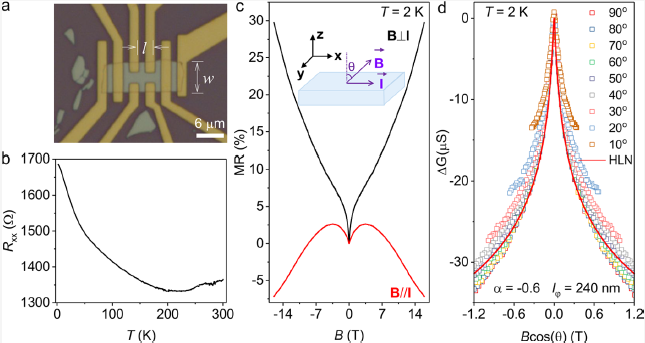
\includegraphics[width=\linewidth]{figures/li_1.png}
\caption{Taken from Fig. 1(a) in~\cite{Li}.(a) The Hall-bar used for the measurements. It has a width of $w\approx 6.7\,\mu\text{m}$ and contact spacing of length $l\approx 2\,\mu\text{m}$.(b) Measured resistance $R$ as a function of temperature $T$ at zero magnetic field $B$.(c) Magnetoresistance measured at $T=2\,$K with $B$ applied from $\theta=0^\circ$ to $\theta=90^\circ$ (see inset).(d) Magnetoconductance as a function of the normal $B$ component, here the solid red line is a fit acquired using the HLN model.}
\label{fig:li_1}
\end{figure}
\begin{figure}[h]
\centering
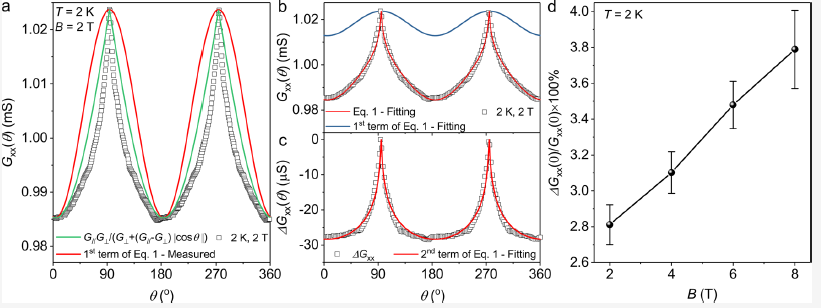
\includegraphics[width=\linewidth]{figures/li_2.png}
\caption{Taken from Fig.2 in~\cite{Li}.(a) Angular dependence of the longitudinal sheet conductance $G_{xx}$ at $B = 2\,$T and $T = 2\,$K. Fit of the conventional AMC using $\frac{G_\parallel G_\perp}{G_\perp+(G_\parallel-G_\perp)|\cos(\theta)|}$ (green) using and fit using with the measured $G_\perp$ and $G_\parallel$ (red line).(b) Angular dependence of $G_{xx}$ at $B=2\,$T and $T=2\,$K. Fit using first term of eq.~\ref{proposedG_xx} with $B_\perp=1.012\,$mS, $\alpha = -0.59$ and $l_\phi = 163\,$nm (red line) and fit of the first term of eq.~\ref{proposedG_xx} using measured $G_\parallel$ value and fitted $G_\perp$ value of about 1.012 mS.(c) Extracted surface state contribution $\Delta G_{xx}$ (points) with HLN model fit (red, Eq.~\ref{HLN}).(d) Magnetic field dependence of surface state contribution ratio $\frac{\Delta G_{xx}(0)}{G_{xx}(0)} \times 100\%$.}
\label{fig:li_2}
\end{figure}
In conclusion the work by Li \textit{et al.}\@ provides a robust method to eliminate the bulk contributions to WAL magnetoconductance-corrections and isolate the surface contributions. 


\section{QHE Experiments}
\begin{figure}[h]
\centering
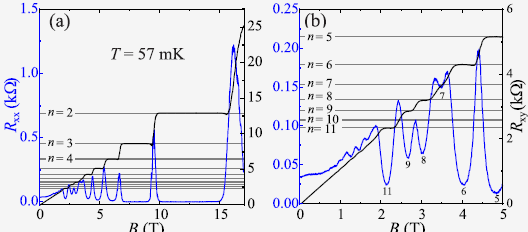
\includegraphics[width=0.45\textwidth]{figures/hartl_hall_resistance.png}
\caption{Hall resistance measured by Hartl \textit{et al.} (Fig. 3(a+b) in~\cite{Hartl}).(a) Measurements at high magnetic field show well quantized plateaus of $R_{xy}$ and vanishing $R_{xx}$.(b) Measurements at lower magnetic fields show small plateaus in $R_{xy}$ and $R_{xx}$ only drops down to a local minima, whenever $R_{xy}$ is plateauing.}
\label{fig:hartl_hall_resistance}
\end{figure}
\label{sec:QHE exp}
The first QHE-focused paper is the recent work done by Hartl \textit{et al.}~\cite{Hartl}. This study focuses on the QHE in the 3DTI HgTe, where multiple types of charge carriers, namely bulk electrons and bulk holes, along surface electrons, are present. The contribution of the various charge carriers to the electronic transport can be studied through their different reactions to an applied gate voltage $V_g$. The sample used can be seen in Fig.~\ref{fig:hartl_sample}. The straining of the HgTe film is crucial as it opens a bulk band gap, enabling HgTe to act as a 3D TI with topological Dirac surface states. Probing the capacitance, in particular probes the top HgTe surface only, therefore isolating the top surface DOS (Ref.\@[12,27] in~\cite{Hartl}).  

Figure~\ref{fig:hartl_hall_resistance}(a) shows Hall resistance measurements taken at $T = 57,$mK. Clear quantum Hall plateaus appear in $R_{xy}$, accompanied by vanishing $R_{xx}$, indicating dissipationless edge transport in these regimes. This implies the surface 2DES dictates transport in these regimes. The authors observe LL filling factors (compare Sec.~\ref{sec:QHE}) $\nu=2,3$ along with Shubnikov-de Haas (SdH) oscillations. Whenever $R_{xx}$ spikes, half-filled LLs, corresponding to a maximum in the DOS, are expected, consistent with the quantum oscillations. For lower magnetic fields, some of the plateaus ($\nu=10,7$) exhibit irregularities (compare Fig.~\ref{fig:hartl_hall_resistance}(b)). The authors attribute this to the distinct evolution of Landau levels for different charge carrier species, which leads to a complex interplay at low magnetic fields. By applying fast Fourier transform (FFT) to the SdH oscillations at low magnetic fields, the authors can distinguish several frequency components associated with different Fermi surfaces. This in turn enables them to distinguish between bulk and surface contributions.  
\begin{figure}[h]
\centering
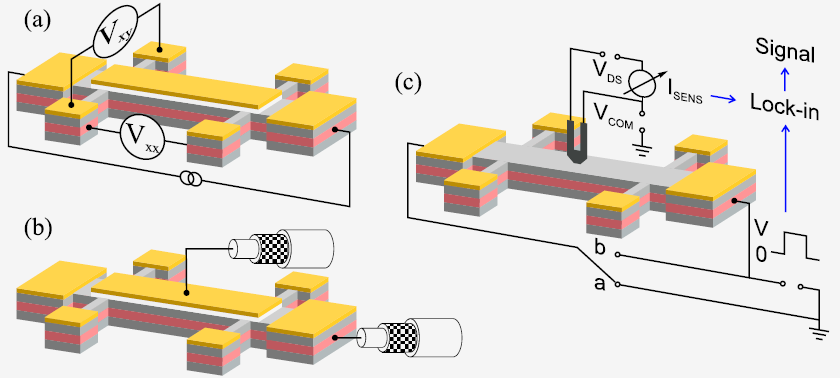
\includegraphics[width=\linewidth]{figures/Hartl_sample.png}
\caption{The heterostructure used in the work done by Hart \textit{et al.}, taken from~\cite{Hartl} Fig. 1(b). (a)The sample used is a heterostructure grown on a (013)-$GaAs$, featuring an 80 nm thick strained HgTe film embedded between cladding layers of CdHgTe (see Fig~\ref{fig:hartl_sample}). Cladding layers of $20 \, nm$ Cd$_{0.68}$Hg$_{0.32}$Te below and $20 \, nm$ thick Cd$_{0.60}$Hg$_{0.40}$Te above HgTe are doped with $10^{17} \, cm^{-3}$. (b)Schematic of the capacitance measurements with $V_{AC}$ (indicated by the coaxial cables) on top of $V_g$. (c)Schematic of the sensitive scanning probe microscopopy. $V_{com}$ indicates a voltage used to compensate a potential difference.}
\label{fig:hartl_sample}
\end{figure}
Capacitance measurements are performed by applying a small AC voltage $V_{AC}$ superposed to a DC gate voltage $V_g$ between the top gate and the HgTe layer. This setup enables extraction of the total capacitance $C$, which consists of both a geometric and a quantum part, $C_{geo}$ and $C_q=e^2\mathrm{DOS}$ respectively. The geometric capacitance depends on the dimensionalities of the device, while the quantum capacitance reflects the density of states (DOS), at the Fermi level of the conductor facing the metallic top gate. The total capacitance is then given by $C^{-1}=C^{-1}_{geo} + C^{-1}_q$.
\begin{figure}[h]
\centering
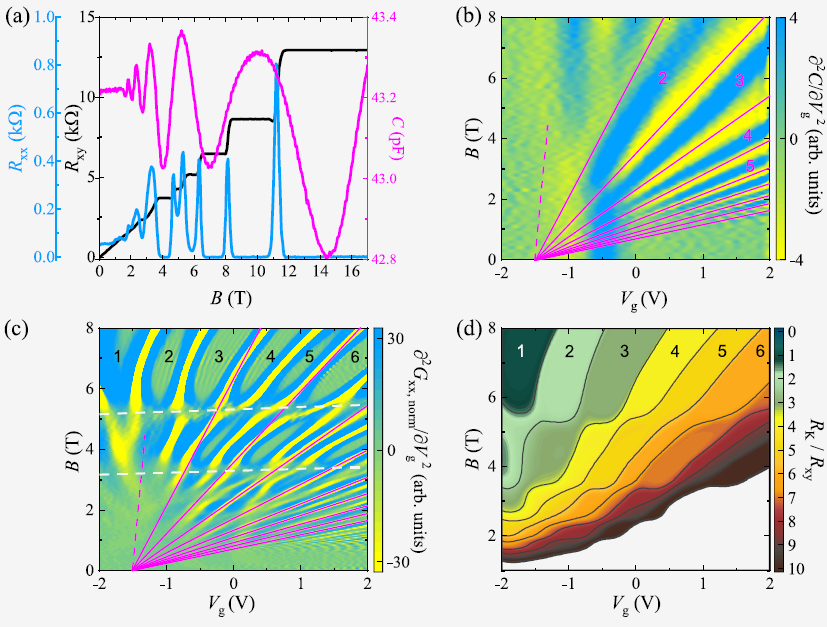
\includegraphics[width=\linewidth]{figures/hartl_comparison.png}
\caption{Taken from Fig.\@5 Hartl \textit{et al.}\@~\cite{Hartl}.(a) Comparison of the capacitance measurements (blue) and the quantum Hall measurements (red) for varying magnetic field $B$, both measured at a gate voltage $V_g=0.5\,$V. (b)Second derivative of the capacitance $C$ with respect to $V_g$ for varying $B$ and $V_g$. Here yellow corresponds to a maximum, implying a maximum in DOS (same for (c)).(c) Second derivative of the conductance $G_{xx}$ with respect to $V_g$ for varying $B$ and $V_g$.(d) }
\label{fig:hartl_comparison}
\end{figure}
To enhance visibility of the structure in the DOS and the authors analyze the second derivatives of the capacitance and magnetoconductance with respect to the gate voltage ($\partial^2 C/\partial V_g^2, \partial^2 G_{xx}/\partial V_g^2$ respectively). The authors then compare the Hall measurements with the capacitance measurements. Since the capacitance measurements are argued to only probe the top surface, there should be clear differences in both measurement techniques. As can be seen in Fig.\@~\ref{fig:hartl_comparison}(b) and (c), the capacitance data shows a clear linear behavior, while the Hall data is more complex. This undermines th

\begin{figure}[h]
\centering
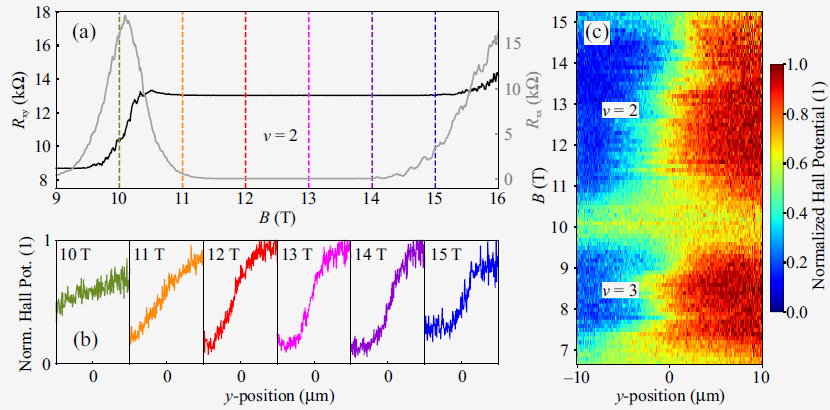
\includegraphics[width=\linewidth]{figures/hartl_spatial.png}
\caption{Taken from Fig. 7 in~\cite{Hartl}.(a) $R_{xx}$ and $R_{xy}$ measured at $T=40\,$mK and a bias voltage of $V_{DS}=0.3\,$mV.(b) Hall potential normalized to $V_{DS}$ for the $\nu=2$ plateau.(c) Hall potentials for different positions of the Hall bar and different magnetic fields.}
\label{fig:hartl_spatial}
\end{figure}

In the final part of their study the authors address the current distribution in the quantum Hall regime, using a scanning probe microscope sensitive to electrostatic potential variations (see Fig.\@~\ref{fig:hartl_sample}). This allows them to measures the local Hall voltage drop over the cross section of an ungated Hall bar with a width of $20\,\mu$m at $T=40\,$mK. With this they can map the Hall potential across the 2DES. At low magnetic fields ($B=10\,$T), consistent with expectations, they observe the classical Hall effect, which is seen from the linear behavior (compare Fig.\@~\ref{fig:hartl_spatial}(b)). Linear behavior implies bulk transport, since arises from current flow through the entire cross section of the sample. However as the magnetic field increases ($B\geq12\,$T) the longitudinal resistance $R_{xx}$ vanishes, indicating a quantum Hall plateau. In contrast to $GaAs/Al_{0.33}Ga_{0.66}AS$ heterostructures, where the Hall voltage drops at the edges of the sample~\cite{WEITZ2000247}, the authors find that their strained HgTe heterostructure has no such edge depletion. Instead they find the voltage drops in the center of the sample, for magnetic fields ranging from $12$-$14\,$T (compare Fig.\@~\ref{fig:hartl_spatial}(b)). They explain this behavior by a central incompressible strip, that forms when the surface channels merge as the magnetic field is raised. 
The work by Hartl \textit{et al.}\@ shows how capacitance measurements enable sole probing of the top surface of a strained HgTe heterostructure, which they demonstrate by comparing capacitance data with conventional quantum Hall resistance measurements. They also use scanning probe microscopy to spatially resolve the currents distribution across the sample. Contrary to $GaAs/Al_{0.33}Ga_{0.66}AS$ heterostructures, they find that the formation of edge channels is suppressed, while the dissipationless current is driven by a voltage drop in incompressible regions of the 2DES.
\begin{figure}[h]
\centering
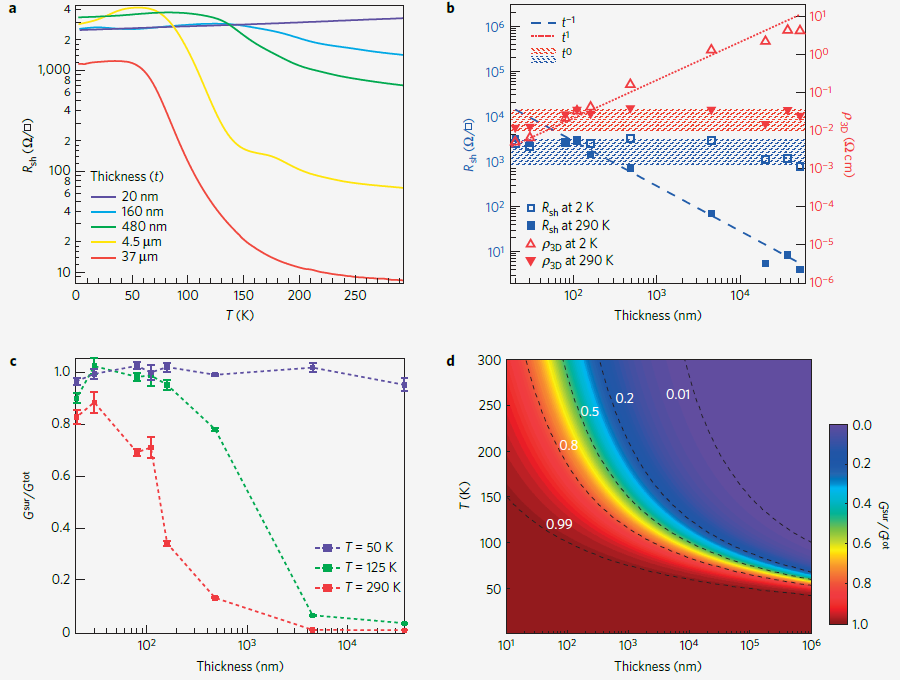
\includegraphics[width=\linewidth]{figures/xu_1.png}
\caption{Taken from Fig.\@1 in~\cite{Xu_2014}.(a) Temperature dependence measurements of the sheet resistance $R_{sh}$ for various thicknesses $t$ at $B=0$.(b) $R_{sh}$ and 3D resistivity $\rho_{3D}$ measurements over $t$ at $T=2\,$K and $T=290\,$K. The dashed line and band correspond to the theoretically expected values for a 3D bulk conductor.(c) Surface conductance $G_{surf}$ divided by total conductance $G_{tot}$ as functions of $t$.(d) Predicted $G_{surf}/G_{tot}$ as function of temperature and thickness, where the respective conductance values are calculated by based on the average conductivities of the bulk and surface.}
\label{fig:xu_1}
\end{figure}

The last experiment to be discussed is the work done by Xu \textit{et al.}\@~\cite{Xu_2014}. The authors study the zero-field transport and the QHE on a BiSbTeSe$_2$ (BSTS) sample, grown via Bridgman technique, for which they observe well-developed topological surface states and a highly insulating bulk. This observation is accompanied by vanishing $R_{xx}$ with quantized Hall conductivity $\sigma_{xy}=\nu e^2/h$ (compare Sec.~\ref{sec:QHE}) for high magnetic fields.
Firstly the authors measure the thickness ($t$) dependence of the quantum Hall transport in the BSTS sample at zero magnetic field (see Fig.\@~\ref{fig:xu_1}). They find that the thicker samples (like $t=37\,\mu$m) show insulating behavior for high temperatures, that shifts to higher temperatures and weakens as $t$ is decreased. Additionally at low temperatures the thicker samples they observe weakly metallic behavior , which the authors attribute to residual bulk carriers freezing out as the temperature lowers. As the sample thickness decreases the temperature range, where the material shows metallic behavior, widens, until at $t=20\,$nm the sample is metallic over the entire temperature range measured (compare Fig.\@~\ref{fig:xu_1}(a)). Furthermore the $T$-dependence of $R_{sh}$ shows differences in the low and high $T$ cases. For high temperatures ($T\geq250\,$K) the values of $R_{sh}$ lie in the range of $<10\,\Omega$ to $>2\,k\Omega$ depending on sample thickness. This behavior reflects the activated bulk conduction and dependence on the cross-section of the sample, which follows $R_{sh}\propto 1/t$. In contrast, for low temperatures $T<50\,$K the authors find $R_{sh}$ is in the range of a few k$\Omega$s and only weakly depend on $t$ (compare Fig.\@~\ref{fig:xu_1} (b)). They attribute this to surface conduction, since the sheet conduction is expected to be essentially independent of $t$. For comparison, the WAL study by García-Abad \textit{et al.}\@shows a similar thickness and temperature dependence in BSTS thin films, where at a certain temperature the thermal activation of phonons cause dephasing of the carriers~\cite{nano11051077}. 
\begin{figure}[h]
\centering
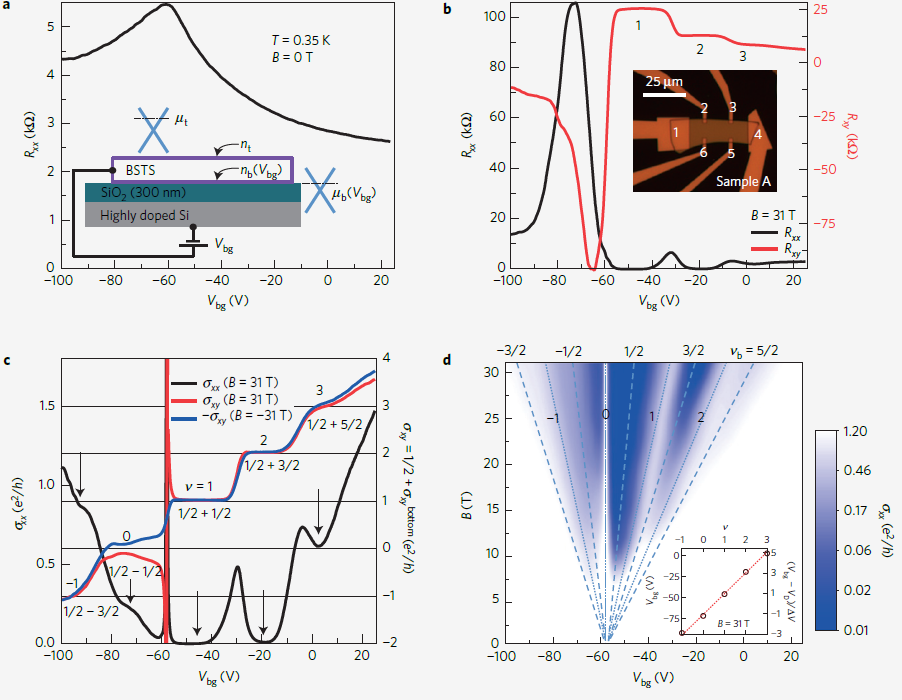
\includegraphics[width=\linewidth]{figures/xu_2.png}
\caption{Taken from Fig.\@ 2 in~\cite{Xu_2014}.(a) Field effect measurement showing $R_{xx}$ as a function of the back gate voltage $V_{bg}$, for a $t=160\,$nm thick sample. Inset shows a schematic of the setup.(b) Hall resistance $R_{xy}$ and longitudinal resistance $R_{xx}$ measured at $B=31\,$T as a function of $V_{bg}$. Inset shows an optical microscope image of the device.(c) 2D longitudinal conductivity $\sigma_{xx}$ and Hall conductivity $\sigma_{xy}$ as functions of $V_{bg}$.(d) $\sigma_{xx}$ as a function of $V{bg}$ and $B$ measured at $T=0.35\,$K.}
\label{fig:xu_2}
\end{figure}
To further analyze their data the authors use a model for the total conductance $G_{tot} = 1/R_{sh}(T)$ to analyze their data. Within this model the conductance is given as the parallel sum of a thermally activated bulk conductance $G_{b}(T)=t\left(\rho_0 \exp^{\Delta/k_b T}\right)$, with the Boltzmann constant $k_b$, the fitting parameter $\rho_0$ and the activation energy $\Delta$ and a metallic surface conductance $G_{surf}(T)= (R_{sh,0} + AT)^{-1}$, with the fitting parameter $R_{sh,0}$, representing low-$T$ residual resistance and the parameter A, reflecting electron-phonon scattering~\cite{Xu_2014}. With this model the authors calculate $G_{sur}$ and compare it to their measured $G_{tot}$ for different $t$ (see Fig.\@~\ref{fig:xu_1} (c)). The behaviour of $G_{sur}/G_{tot}$ further manifests the thickness independence at low-$T$ and therefore the dominant surface conduction, which, for $t<100\,$nm, even shows significant contribution even at room temperatures. 
Afterwards they conduct QHE measurements for two samples of thicknesses $t=160\,nm$ and $t=80\,$nm, respectively. Their measurement setup enables them to tune only the bottom surface carrier density $n_b$, leaving the top surface carrier density $n_t$ unaffected. The back gate voltage $V_{bg}$ is modulated via a $Si/SiO_2$ backgate. The charge neutrality point (CNP) is identified at $V_{CNP}=-60\,$V, indicating transport by electrons for $V_{bg}>-60\,$V and holes transport by holes for $V_{bg}<-60\,$V (compare Fig.\@~\ref{fig:xu_2}(a)). In Fig.\@~\ref{fig:xu_2}(b) the longitudinal resistance $R_{xx}$ is shown as a function of $V_{bg}$, where a magnetic field of $B_31\,$T is applied. In the electron regime ($V_{bg}>V_{CNP}$), the QHE is observed, manifesting itself by regions in which $R_{xy}$ is quantized and where $R_{xx}$ vanishes. The authors found LL filling factors to be $\nu=1$ for the thicker sample and $\nu=2$ for the thinner sample. In Fig.\@~\ref{fig:xu_2}(c) the longitudinal conductivity $\sigma_{xx}$ and the Hall conductivity $\sigma_{xy}$ are computed by tensor inversion and shown as a function of $V_{bg}$. Once again the authors find behaviour typically associated with the QHE (plateaus in $\sigma_{xy}$ where $\sigma_{xx}$ vanishes), with associated $\nu=1,2,3$, where for the third plateau, $\sigma{xx}$ only goes to a minimal value. The authors conclude that the associated integer filling factors is given by the sum of two half-integer filling factors stemming from the top surface (with $\nu=1/2$) and bottom surface (with $\nu=1/2,3/2,\cdots$ depending on $V_{bg}$) respectively. This once more clearly indicates surface transport regimes.
\begin{figure}[h]
\centering
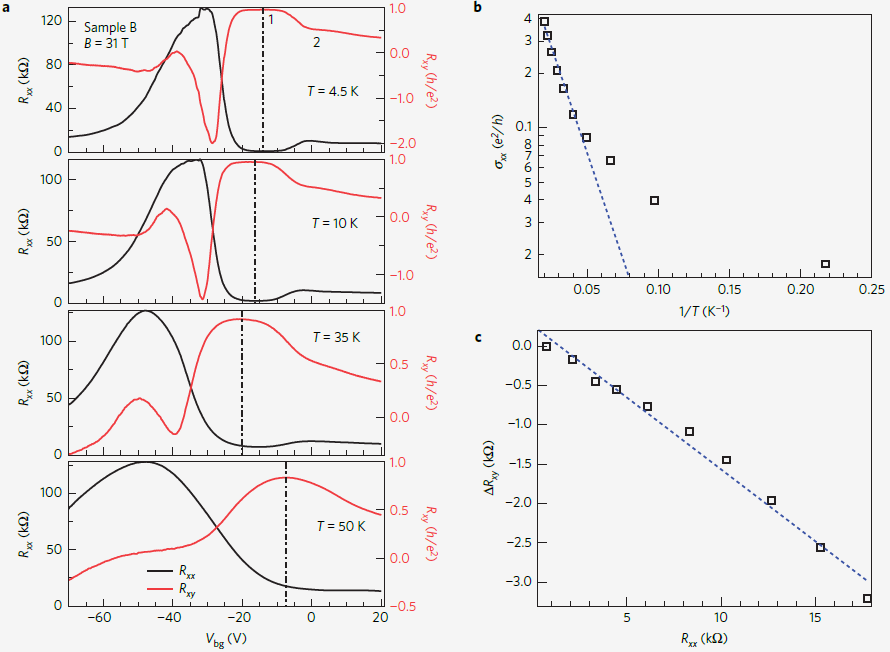
\includegraphics[width=0.9\linewidth]{figures/xu_3.png}
\caption{Taken form Fig.\@ 4 in~\cite{Xu_2014}.(a) Measurements of Hall resistivity $R_{xy}$ and longitudinal resistivity $R_{xx}$, performed on the 80nm thick sample, as a function of back gate voltage $V_{bg}$ for several temperatures $T$ at a magnetic field strength of $B=31\,$T.(b) Fit of the longitudinal conductivity $\sigma{xx}$ as a function of inverse temperature $1/T$ for $\nu=1$ (blue dashed line is a fit for higher $T$).(c) $\Delta R_{xy}(T)=R_{xy}(T) - R_{xy}(T=4.5\,K)$ versus $R_{xx}$ for $\nu=1$ (blue dashed line is a linear fit)}
\label{fig:xu_3}
\end{figure}
Afterwards the authors performed measurements of $R_{xy}$ and $R_{xx}$, on the sample with $t=80\,$nm at $B=31\,$T, for temperatures $T=4.5, 10, 35 \mathrm{and} 50\,$K respectively (see Fig.\@~\ref{fig:xu_3}(a)). Again plateaus can be see, which the authors associate with $\nu=1$ and $\nu=2$, while the second plateau is not fully developed yet. As the temperature is increased the authors observe, that at $T=10\,$K the plateaus start to weaken and disappear at around 50K. Furthermore the authors study the $T$-dependence of the conductivity and that of $\Delta R_{xy}(T) = R_{xy}(T) - R_{xy}(T=4.5\,\mathrm{K})$ (see Fig.~\ref{fig:xu_3}(b)+(c) respectively). They find that the activation gap is significantly smaller than the theoretically expected one, which they attribute to disorders, that in turn lead to LL broadening, and the effects of their finite side surface. Also they show linear $T$-dependence of $\Delta R_{xy}(T)$, which was commonly observed in 2DES~\cite{Matthews2005}. 

In conclusion, Xu \textit{et al.} conduct a study of both zero-field and quantum Hall transport, showing a transition from surface conduction to bulk conduction, in the 3DTI BiSbTeSe$_2$ (BSTS). In high magnetic fields they observe quantized Hall plateaus and vanishing longitudinal resistances in samples of thicknesses $t=80\,$nm and $t=160\,$nm respectively, consistent with the characteristics of the QHE. By  gating the bottom surface, they demonstrate quantized Hall conductance arising from combined top surface and bottom surface Dirac fermions, with integer $\nu$, reflecting the sum of two half-integer channels. These findings are comparable to WAL experiments on the same material. 

\section{Further Discussion and Conclusion}
The reviewed experiments give an overview of quantum transport in 3DTIs and provide evidence for topological surface states in 3DTIs. Despite differences in material composition, sample geometry and fabrication techniques, these experiments consistently demonstrate significant contribution to electronic transport from topological surface states, under certain conditions. The strengths to isolate the surface carrier contributions from the bulk carrier contributions, is compared between all studies. 
The choice of material plays an important role when trying to isolate the surface from the bulk transport. Li \textit{et al.} and Xu \textit{et al.} both employ samples made out of BiSbTe$_2$, which possess a higher bulk resistivity compared to Bi$_2$Se$_3$, which is investigated by García-Abad \textit{et al.} The work by Hartl \textit{et al.} uses a strained HgTe heterostructure to create a sufficiently high bulk gap, to enable topological states. Fabrication methods are similarly crucial. MBE used for Bi$_2$Se$_3$ allows for controlling sample thickness, enabling García-Abad \textit{et al.} to study the crossover from bulk dominated transport in thick films to surface dominated transport in films thinner than $\approx$10 QL and additionally study the thickness dependence in that material. In contrast, the Bridgman technique used by Xu \textit{et al.} produces high quality BiSbTeSe$_2$ bulk crystals, from which thin flakes ($t<500\,$nm), where the bulk is highly insulating, can be exfoliated.

In the analysis of WAL the parameter $\alpha$ in the HLN model serves as a measure of the number of conducting channels. In an ideal case of two perfectly decoupled surfaces in thin films, $\alpha$ approaches -1, where each surface contributes with $\alpha=-0.5$. However, the more common observation of $\alpha \approx -0.5$ indicates top and bottom surfaces are coupled through the bulk, causing them to behave as a single dominant channel. García-Abad \textit{et al.} show evolution from $\alpha \approx -1/2$ in bulk coupled or single surface systems towards $\alpha = -1$ in the less disordered, thinner samples. This matches the expectation of uncoupled surfaces for clean and thin samples. Li \textit{et al.} improve this approach by using the anisotropic magnetoconductance to separate the 2D WAL signal (surface contribution) from the 3D bulk signal. After subtracting the anomalous magnetoconductance (bulk contribution), they extract $\alpha \approx -0.59$, consistent with a single channel formed by the surfaces coupled through the bulk. In the work by Xu \textit{et al.} on BiSbTeSe$_2$ they use a back gate to tune the carrier density of the bottom surface, while assuming the top surface remains fixed at its lowest half-integer LL ($\nu_{t}=1/2$). The authors demonstrate well developed quantum Hall plateaus in $\sigma_{xy}$ and vanishing longitudinal conductivity $\sigma_{xx}$ for integer filling factors $\nu=1, 2, 3$. They conclude, that these integer plateaus arise as the sum of two half-integer channels ($\nu = \nu_\mathrm{t} + \nu_\mathrm{b}$), corresponding to the top and bottom surfaces respectively. Hartl \textit{et al.} advance this by studying a strained HgTe heterostructure, where they perform transport and capacitance measurements. Since the capacitance measurement probes only the density of states of the top surface facing the gate, they can independently track its LLs and directly compare them to the transport measurements taken on the whole sample (top, bottom and bulk). Furthermore Hartl \textit{et al.} employ scanning probe microscopy to spatially map the Hall potential, revealing that Hall potentials do not drop at the edges of the sample, but rather across a broad region in the interior. They explain this behavior by a current that's not confined to dissipationless edge channels, but instead flows through an extended region within the sample. They interpret this behavior not as proof of absent edge modes, but as evidence that multiple electronic subsystems merge into a single, spatially extended conduction channel under high magnetic fields.
In summary, the complementary approaches of WAL and QHE measurements provide robust experimental verification of topological surface states in 3DTIs, despite the challenges posed by bulk contributions. Future advancements in material growth and device fabrication, providing cleaner samples, will likely enable even better isolation of surface transport, paving the way for topological quantum applications.
\bibliographystyle{unsrt}
\bibliography{refs}
\end{document}